\chapter*{Exploratory Data Analysis}\label{chap:eda}
An extensive analysis of the data that will be used during the development process was carried out. This chapter presents the results of this analysis, which are used to guide the development of the system.


\section{Preliminary Analysis}\label{sec:data_prelim_analysis}
The data used by MULTI-VP and, consequently, the RNN prediction model consists of magnetogram data from the Wilcox Solar Observatory. Each file contains 12 columns representing measurements of the magnetic field in the solar atmosphere at different heights. Every variable comprises 640 points (abscissas) measured at different radial distances from the Sun (up to 30 Solar radii). For this work, only six columns will be used, as the others are derivations of these and, thus, are significantly correlated. 

The data columns can be seen in Table \ref{tab:multivp_columns}. These are divided into two parts: the input and the output. The former comprises the set of variables used by the simulation to approximate solar wind conditions, while the former consists of the initial expert guesses needed to kickstart the multiple flux simulation. The input data comprises the magnetic field amplitude, $B$, the flux tube inclination, $\alpha$, and the radial coordinate, $R$. The output data includes the number of charged particles per unit volume, $n$, the velocity, $v$, and the temperature, $T$.

\begin{table}[ht]
    \caption{Data columns of magnetogram used by MULTI-VP.}
    \label{tab:multivp_columns}
    \begin{subtable}[h]{0.32\textwidth}
        \centering
        \begin{tabular}{lcc}
        \hline
        \multicolumn{3}{c}{Input (Partial Flows)}                              \\ \hline
        $R${[}$R_{sun}${]} & $B${[}$G${]} & $\alpha${[}$deg${]} \\ \hline
        \end{tabular}
    \end{subtable}
    \begin{subtable}[h]{0.32\textwidth}
        \centering
        \begin{tabular}{ccc}
        \hline
        \multicolumn{3}{c}{Output (Estimations)}                           \\ \hline
        $n${[}$cm^{-3}${]} & $v${[}$km/s${]} & $T${[}$MK${]} \\ \hline
        \end{tabular}
    \end{subtable}
\end{table}

A joint plot of the input variables can be seen in Fig. \ref{fig:jointplot_input}. From these plots, it can be concluded that several input files constitute anomalous data. This is clear from the graphs of $B$ and $\alpha$, with files that significantly deviate from the rest.


\begin{figure}[h]
    \centering
    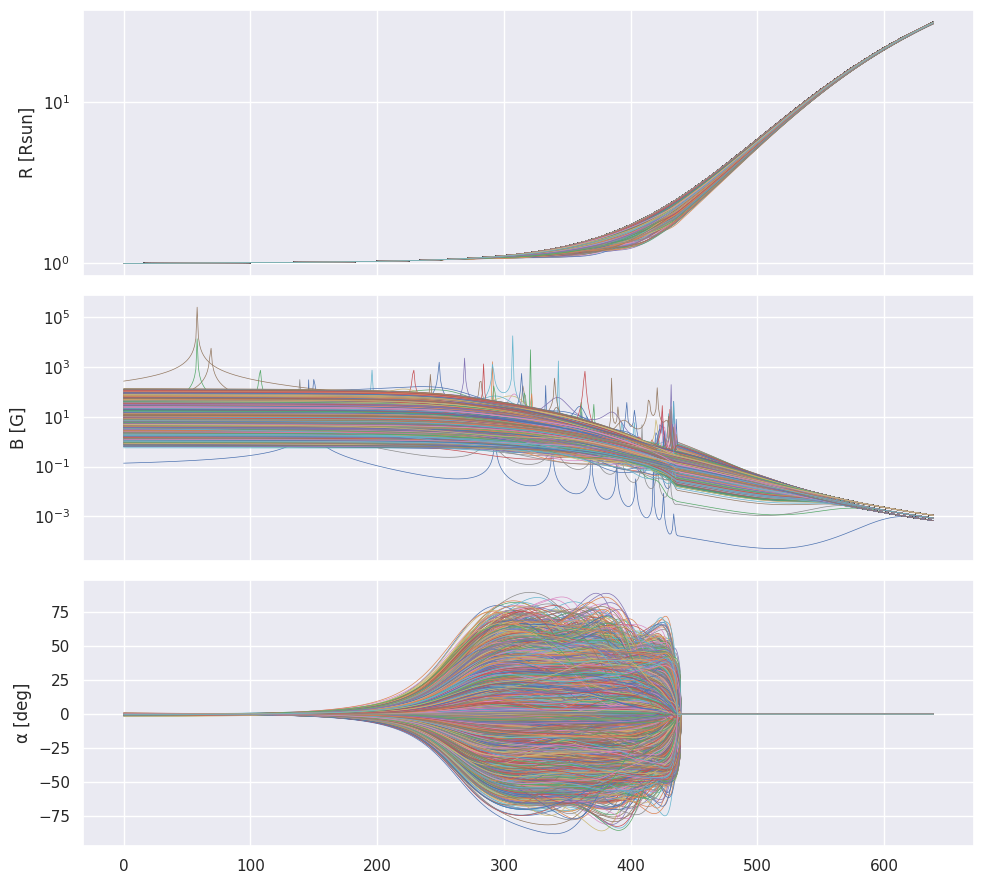
\includegraphics[width=0.8\textwidth]{figures/joint_input_cols.png}
    \caption{Joint plot of the input variables of each file used in this work. The first row is the plot of the radial coordinate radius, $R$, the second the magnetic field, $B$, and the last the flux tube inclination $\alpha$. All are plotted in function of position in the magnetogram file.}
    \label{fig:jointplot_input}
\end{figure}

% TODO refs para research statement
As previously explained, MULTI-VP requires initial expert guesses to kickstart the simulation. These guesses consist of the output variables presented in Table \ref{tab:multivp_columns} and, during the simulation, are approximated to better solutions. In line with the work carried out in \cite{barros_InitialConditionEstimation_}, we will be using the outputs of previous simulations as initial guesses (refer to chapter \ref{chap:research_proposal} for more details).


Fig. \ref{fig:jointplot_output} shows the joint plot of the output variables. Similar to the input plots, several faulty predictions can be seen in all variable plots, which are the result of simulations carried out on anomalous inputs.

\begin{figure}[h]
    \centering
    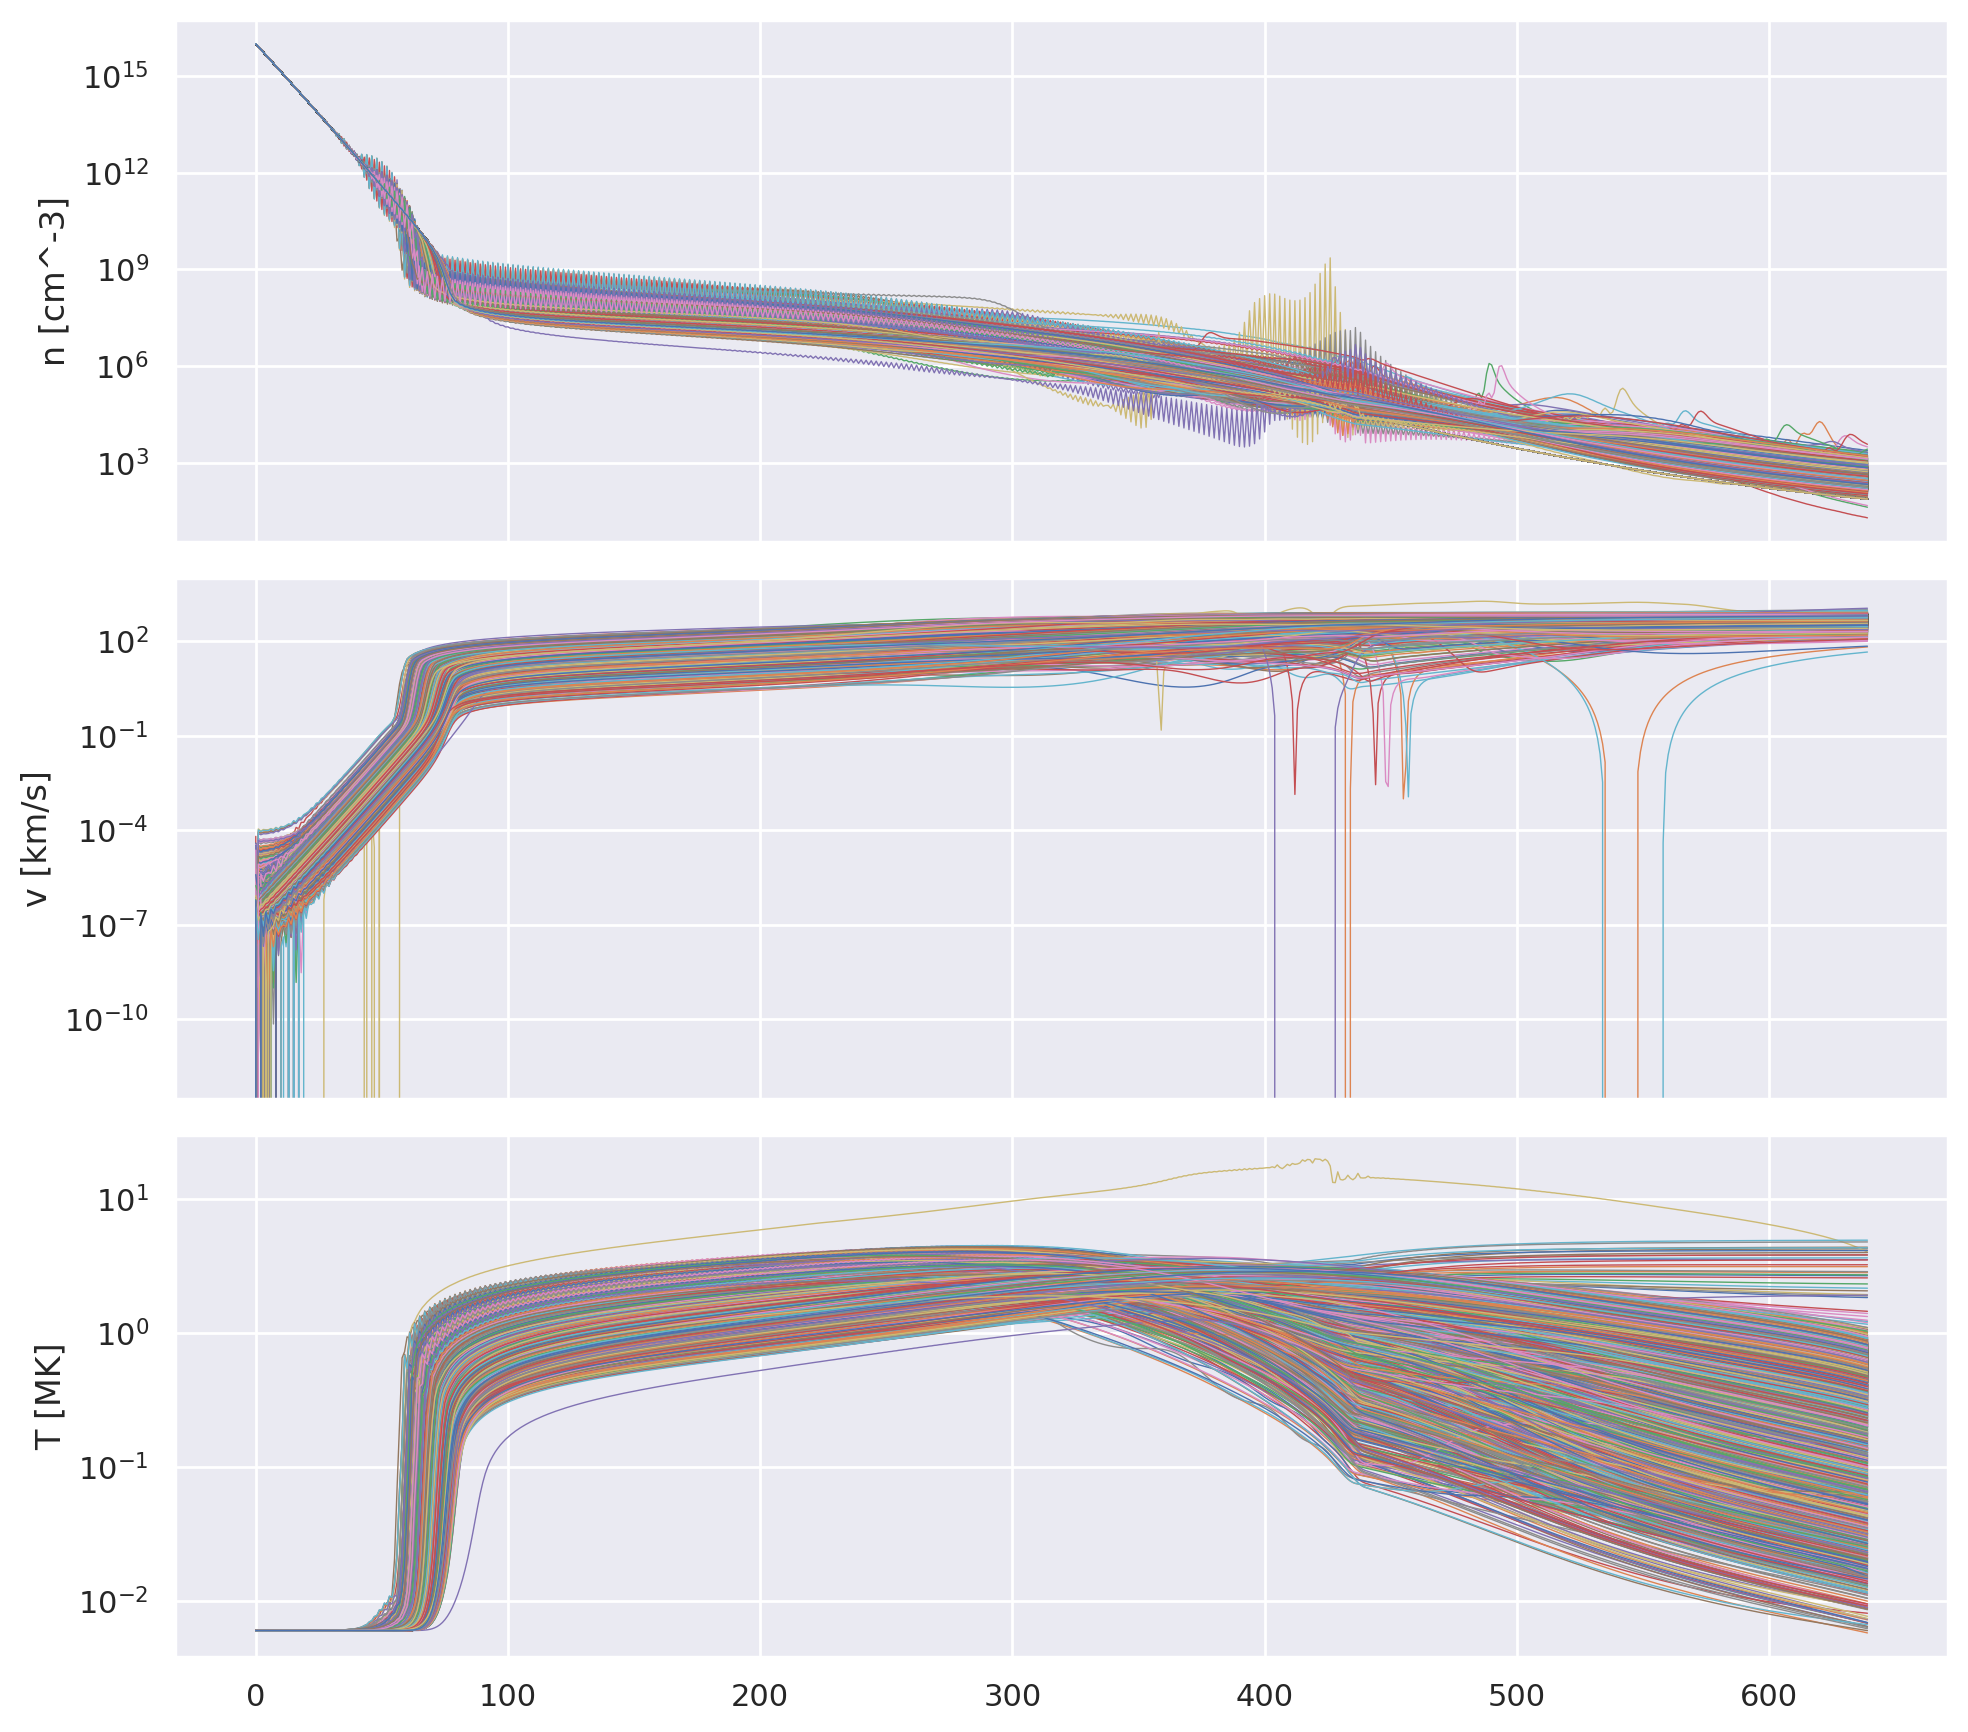
\includegraphics[width=0.8\textwidth]{figures/joint_output_cols.png}
    \caption{Joint plot of the output variables of each file used in this work. The first row is the plot of the number of charged particles per unit volume, $n$, the second the velocity, $v$, and the last the temperature, $T$. All are plotted in function of position in the magnetogram file.}
    \label{fig:jointplot_output}
\end{figure}

A preliminary statistical analysis of the data can be seen in tables \ref{tab:data_stats}. In it, the mean, standard deviation, minimum, maximum, and quartiles of each variable are presented.

\begin{table}[h]
    \caption{Data Statistical Analysis}
    \label{tab:data_stats}
    \begin{tabular}{@{}rrrrrrr@{}}
    \toprule
    \textbf{} & \textbf{R {[}Rsun{]}} & \textbf{B {[}G{]}} & \textbf{alpha {[}deg{]}} & \textbf{n {[}cm\textasciicircum{}-3{]}} & \textbf{v {[}km/s{]}} & \textbf{T {[}MK{]}} \\ \midrule
    mean      & 4.755                 & -0.536             & 1.885                    & 8.630207e+13                            & 255.325               & 1.384               \\
    std       & 7.165                 & 91.948             & 14.728                   & 6.839549e+14                            & 214.855               & 0.897               \\
    min       & 1.000                 & -17541.107         & -87.632                  & 1.972793e+01                            & -0.007                & 0.006               \\
    $25\%$    & 1.021                 & -2.145             & -0.108                   & 1.622396e+04                            & 49.263                & 0.718               \\
    $50\%$    & 1.151                 & 0.001              & 0.000                    & 2.350818e+06                            & 211.022               & 1.337               \\
    $75\%$    & 4.250                 & 2.054              & 1.000                    & 2.131588e+07                            & 450.770               & 2.098               \\
    max       & 31.501                & 247095.581         & 89.257                   & 1.009917e+16                            & 1889.365              & 19.897              \\ \bottomrule
    \end{tabular}
\end{table}